\documentclass[12pt]{article}

\pagestyle{empty}
\setlength{\topmargin}{0in}
\setlength{\headheight}{0in}
\setlength{\topsep}{0in}
\setlength{\textheight}{9in}
\setlength{\oddsidemargin}{0in}
\setlength{\evensidemargin}{0in}
\setlength{\textwidth}{6.5in}

\usepackage{palatino,graphicx,amsmath,amssymb,enumitem}

\newcommand{\ds}{\displaystyle}
\newcommand{\vs}[1]{\vspace{#1in}}
\renewcommand{\vss}[1]{\vspace*{#1in}}
\newcommand{\bvec}{{\mathbf b}}
\newcommand{\cvec}{{\mathbf c}}
\newcommand{\dvec}{{\mathbf d}}
\newcommand{\evec}{{\mathbf e}}
\newcommand{\fvec}{{\mathbf f}}
\newcommand{\qvec}{{\mathbf q}}
\newcommand{\uvec}{{\mathbf u}}
\newcommand{\vvec}{{\mathbf v}}
\newcommand{\wvec}{{\mathbf w}}
\newcommand{\xvec}{{\mathbf x}}
\newcommand{\yvec}{{\mathbf y}}
\newcommand{\zvec}{{\mathbf z}}
\newcommand{\zerovec}{{\mathbf 0}}
\newcommand{\real}{{\mathbb R}}
\newcommand{\twovec}[2]{\left[\begin{array}{r}#1 \\ #2
    \end{array}\right]}
\newcommand{\ctwovec}[2]{\left[\begin{array}{c}#1 \\ #2
   \end{array}\right]}
\newcommand{\threevec}[3]{\left[\begin{array}{r}#1 \\ #2 \\ #3
  \end{array}\right]}
\newcommand{\cthreevec}[3]{\left[\begin{array}{c}#1 \\ #2 \\ #3
    \end{array}\right]}
\newcommand{\fourvec}[4]{\left[\begin{array}{r}#1 \\ #2 \\ #3 \\ #4
    \end{array}\right]}
\newcommand{\fivevec}[5]{\left[\begin{array}{r}#1 \\ #2 \\ #3 \\ #4 \\ #5
    \end{array}\right]}
\newcommand{\cfourvec}[4]{\left[\begin{array}{c}#1 \\ #2 \\ #3 \\ #4
    \end{array}\right]}
\newcommand{\mattwo}[4]{\left[\begin{array}{rr}#1 & #2 \\ #3 & #4 \\ \end{array}\right]}
\renewcommand{\span}[1]{\text{Span}\{#1\}}
\newcommand{\bcal}{{\cal B}}
\newcommand{\ccal}{{\cal C}}
\newcommand{\scal}{{\cal S}}
\newcommand{\wcal}{{\cal W}}
\newcommand{\ecal}{{\cal E}}
\newcommand{\coords}[2]{\left\{#1\right\}_{#2}}
\newcommand{\gray}[1]{\color{gray}{#1}}
\newcommand{\lgray}[1]{\color{lightgray}{#1}}
\newcommand{\rank}{\text{rank}}
\newcommand{\col}{\text{Col}}
\newcommand{\nul}{\text{Nul}}
\newcommand{\bhat}{\widehat{\bvec}}
\newcommand{\xhat}{\widehat{\xvec}}
\newcommand{\xbar}{\overline{\xvec}}
\newcommand{\xtilde}{\widetilde{\xvec}}
\newcommand{\ytilde}{\widetilde{\xvec}}
\newcommand{\len}[1]{\left|#1\right|}
\newcommand{\sighat}{\widehat{\Sigma}}
\newcommand{\code}[1]{\smallskip \\ \noindent{\tt #1} \smallskip
  \\ \noindent} 
\newcommand{\codeend}[1]{\smallskip \\ \noindent{\tt #1}}
\renewcommand{\c}[1]{{\tt #1}}

\begin{document}

\noindent
{\bf Introduction to Sage} \\

\bigskip
Open the page of Sage cells at {\tt gvsu.edu/s/0Ng}.  There is also a
Sage cell server at {\tt https://sagecell.sagemath.org/}.

\begin{itemize}
\item
  In the first cell, enter
  \code{2 + 5}
  and evaluate the cell using either the button below the cell or by
  pressing Shift-Enter.

\item  Still using the first cell, enter \code{2 + 5 \\ 2 * 5} and
  evaluate.

{\bf General principle:}  {\em Sage only reports the result
  of the last operation in a cell.}

\item Try this:
  \codeend{print(2+5) \\ 2 * 5}

\item We can store results using variables: \code{a = 2*5}  Notice
  that Sage finishes silently.  While it does compute \c{2*5}, it then
  assigns the result to \c{a} so the last operation performed in the
  cell is the assigment.  

\item We can check the value of the variable by evaluating
  \codeend{a = 2*5 \\ a}

\item Results obtained in one cell are available in other cells.  In
  the second cell, evaluate
  \codeend{2\^{}a}

\item To define the matrix
  $A = \begin{bmatrix} 1 & 2 & 1 \\ 2 & 1 & 3 \end{bmatrix}$, use
  \code{A = matrix(2, 3, [1, 2, 1, 2, 1, 3])}
  There are three arguments to the \c{matrix} command:  the number of
  rows, the number of columns, and a Python \c{list} consisting of the
  entries read across the rows.
  
  To find the reduced row echelon form, use \codeend{A.rref()}

  {\bf General principle:}  {\em Once you define a \c{thing}, you can
  perform a natural \c{action} on the \c{thing} using
  \code{thing.action()}
  Take note of the open and close parentheses.}
  
\item Now define the matrix 
  $A = \begin{bmatrix} 1.0 & 2 & 1 \\ 2 & 1 & 3 \end{bmatrix}$, taking
  note that one entry has been changed to floating point.  Find the
  reduced row echelon form of $A$.  What do you notice?

  Mathematically, we know these are the same matrices, but Sage views
  the entries of the matrix as elements in a field in which any
  computations are performed.  We don't need to worry about this now;
  just be aware of it.

  Incidentally, you can use
  \codeend{n(A.rref(), digits=3)}
  to modify the appearance of the result.  I didn't show this to
  students in MTH 227.

\item Define the matrix $A = \begin{bmatrix} 1 & 2 \\ 2 &
    1 \end{bmatrix}$.  Vectors may be defined by
  \code{v = vector([3, -2])}
  This is a simple syntax:  just provide a list of the elements of the
  vector.

  To multiply:
  \code{A * v}
  To augment:
  \code{A.augment(v)}
  Operations can be concatenated:
  \codeend{A.augment(v).rref()}

\item We can assemble matrices from vectors:
  \code{v1 = vector([2, -3]) \\ v2 = vector([1,4]) \\ matrix([v1,
    v2])}
  Here we define two vectors and create a matrix using a \c{list} of
  vectors.

  Does this produce what you want?  How can you make it produce what
  we want?  Hint:  \c{thing.action()}.

\item We can also pull vectors out of matrices.  What does this code do?
  \codeend{A = matrix(2, 2, [1, 2, 2, 1]) \\ b = vector([3,0]) \\
    x = A.augment(b).rref().column(2) \\ x}

  {\bf Helpful Python fact:}  {Like most computer languages, Python
    starts counting at \c0 so the third column of a matrix is indexed
    by \c2.}
  
  {\bf Helpful Python trick:}  {\c{A.column(-1)} pulls out the last
    column, \c{A.column(-2)} the next to last column, and so forth.}

\item We can also pull columns out of $A$ into a matrix:
  \code{A = matrix(2, 4, [3,-2,0,4,-1,-1,2,2]) \\
    B = A.matrix\_from\_columns([2, 1])}

\item The $n\times n$ identity matrix is
  \code{I = identity\_matrix(n)}
  Suppose that $A = \begin{bmatrix} 1&2 \\ 2&1 \end{bmatrix}$.
  Evaluate
  \codeend{A - 3*I}

\item {\bf Inverses:}  
  Find $A^{-1}$ using three different methods:

  a) \c{thing.action()}

  b) Augment $A$ to $[~A~|~I~]$, row reduce, and extract.

  c) \c{A\^{}-1}

\item Find the determinant of $A$.

\item Find the eigenvalues of $A$.

\item   To find a basis for the null space $\nul(B)$, use
  \code{B.right\_kernel()}
  Using the matrix $A$ above, find a basis for the eigenspaces $E_3$
  and $E_{-1}$. 

\item Define the stochastic matrix $S = \begin{bmatrix}0.4&0.3 \\
    0.6&0.7 \end{bmatrix}$.  We know that $\lambda=1$ is an
  eigenvalue.  What happens when we try to find $\nul(S-I)$?

  How would you handle this with your students?

\item Go back to $A = \begin{bmatrix} 1 & 2 \\ 2 & 1 \end{bmatrix}$.
  The command
  \code{A.eigenmatrix\_right()}
  attempts to diagonalize $A$ and returns a pair of matrices $D$ and
  $P$.

  To save them, use
  \code{D, P = A.eigenmatrix\_right()}
  Now verify that $A = PDP^{-1}$.

\item What happens when we try to diagonalize $A = \begin{bmatrix} 1 &
    1 \\ 0 & 1 \end{bmatrix}$?

\item {\bf Danger:}  The \c{eigenmatrix\_right} command tries to
  compute exactly in the ring defined by the matrix.
  If you try
  \code{S.eigenmatrix\_right()}
  it will fail.  You instead need to tell Sage to compute in a ring
  called \c{RDF}, which enables floating point approximate
  arithmetic.  Use either
  \code{A = matrix(RDF, 2,2,[0.4,0.3,0.6,0.7]) \\
    A = matrix(RDF, A) \# if A has already been defined}

\item You can create pages with custom commands.  Go to {\tt
    http://gvsu.edu/s/0TD} where you will find a page that contains
  three commands to implement the power method:
  \code{power(A, x, N)}
  iterates the power method $N$ times, with an initial vector $x$,
  giving an approximation to the 
  dominant eigenvalue and a corresponding eigenvector.
  \code{inverse\_power(A, x, N)}
  iterates the inverse power method $N$ times giving an approximation
  to the smallest (in absolute value) eigenvalue and a corresponding
  eigenvector.
  \code{find\_closest\_eigenvalue(A, s, x, N)}
  finds the eigenvalue closest to $s$ and a corresponding eigenvalue.

  Use these commands to find the eigenvalues of the matrix $B$ defined
  on that page.

  \begin{center}
    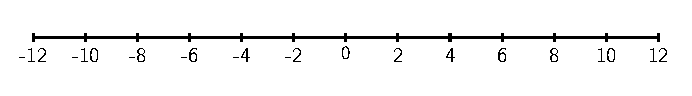
\includegraphics{number-line.eps}
  \end{center}

\item You should learn enough python to write a loop:

  \noindent
  {\tt for i in range(10): \\
  \hspace*{24pt} print(i)}
 
  and to define a function:
  \code{def fibonacci(n): \\
    \hspace*{24pt} if n == 0: return 0 \\
    \hspace*{24pt} if n == 1: return 1 \\
    \hspace*{24pt} return fibonacci(n-1) + fibonacci(n-2)}
    
\end{itemize}

{\bf Quick reference:} There is a useful ``quick reference,'' a 2-page
document outlining 
linear algebra commands in Sage.  To find it, google 
\c{sagemath linear algebra quick reference}

\end{document}

Student reaction has been positive
Natural syntax and easy to learn
lots of ways to use
python based



